\documentclass[11pt,a4paper]{article}
\usepackage[utf8]{inputenc}
\usepackage[T1]{fontenc}
\usepackage[romanian]{babel}
\usepackage{graphicx}
\usepackage[hmargin=2.5cm,vmargin=2.5cm]{geometry}
\usepackage{microtype}
\usepackage{setspace}
\usepackage{hyperref}
\usepackage{caption}

\title{\LARGE\bfseries Abacul roman}
\author{Student 1 \and Student 2}
\date{}

\begin{document}
\maketitle
\begin{center}
\begin{minipage}{0.75\textwidth}
\singlespacing
\noindent\textbf{Disciplina:} Arhitectura sistemelor de calcul / Proiect\\
\textbf{Profesor:} \\
\textbf{Data:} \\
\end{minipage}
\end{center}

\vspace{1cm}

\begin{figure}[h]
  \centering
  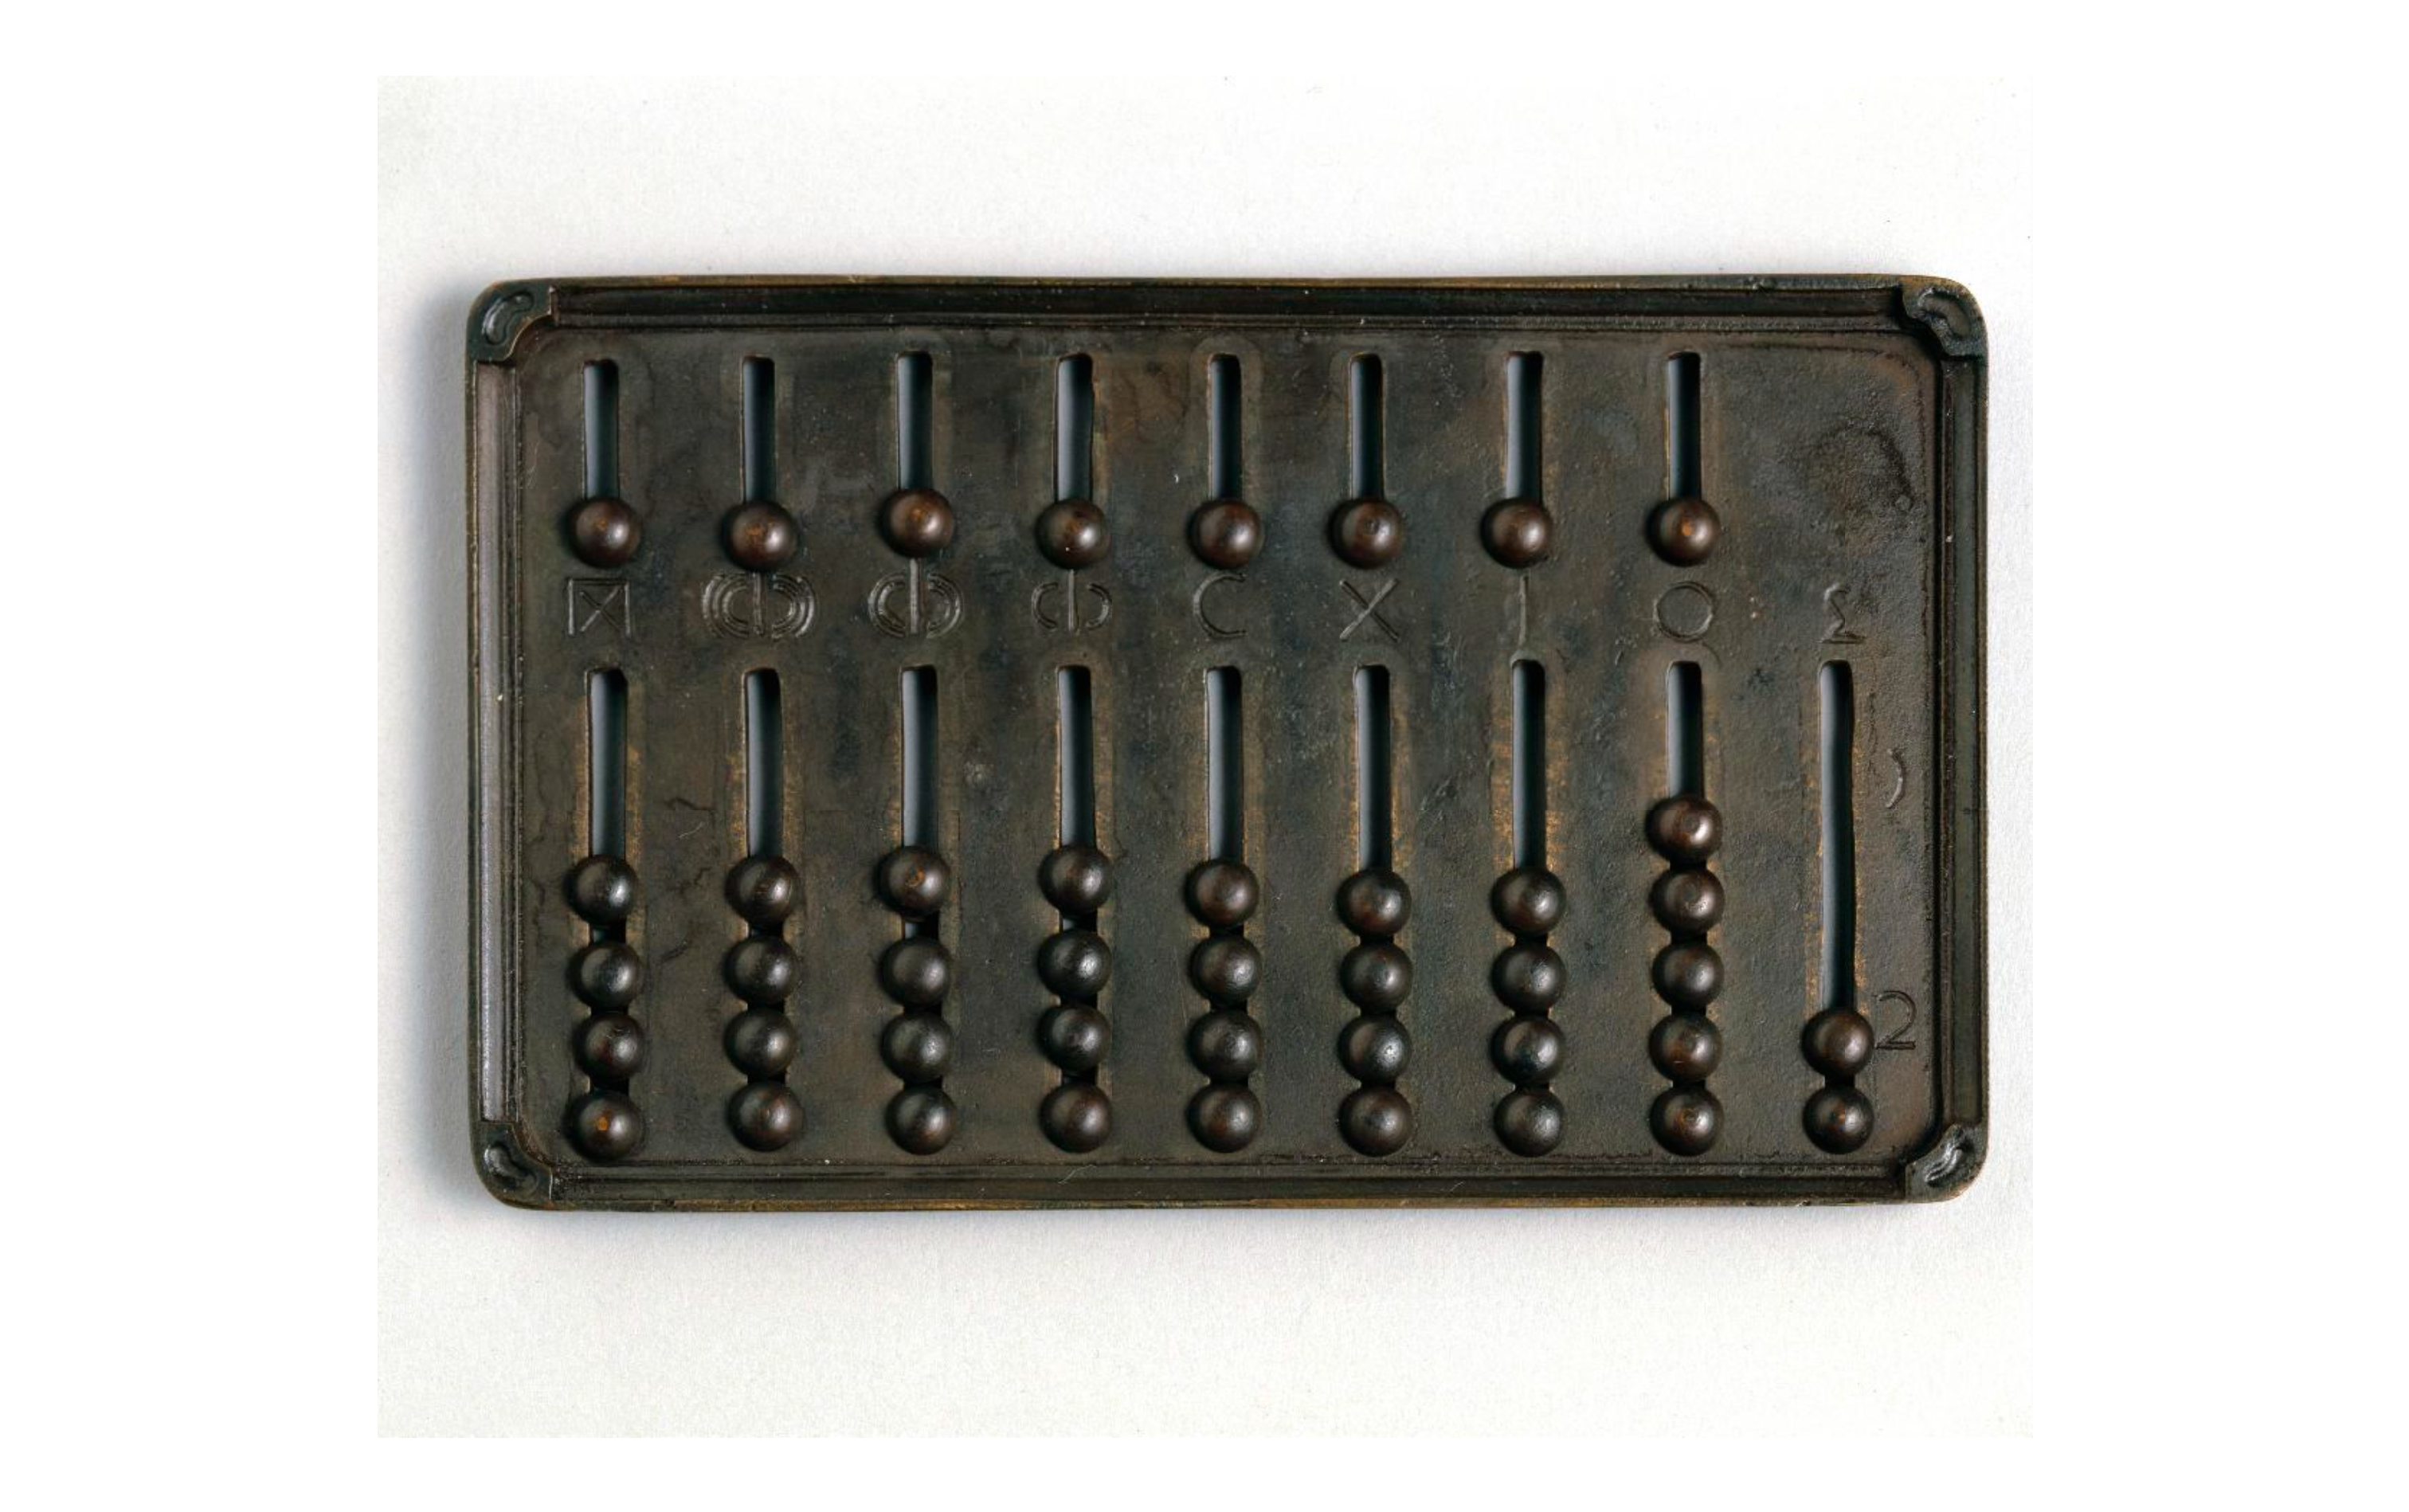
\includegraphics[width=0.6\textwidth]{roman-abacus.png}
  \caption*{Exemplu de abac roman (replică / exemplar bronze). Sursa imaginei: vedeți Bibliografia pentru link direct.}
\end{figure}

\begin{abstract}
Acest eseu analizează abacul roman, un instrument portabil de calcul folosit în lumea romană. Vom descrie structura fizică, principiile de funcționare şi rolul acestuia în practici comerciale şi inginereşti, precum şi influenţele şi importanţa sa istorică. Scopul este de a oferi o prezentare clară şi concisă, adecvată ca proiect şcolar, respectând formatul uzual de eseu.
\end{abstract}

\section*{Introducere}
Abacul roman reprezintă o variantă portabilă a tablelor de numărat folosite în lumea antică, concepută pentru calcule uzuale: adunare, scădere, operaţii cu fracţii şi evidenţa contabilă. Deşi scrierea numerică romană nu includea un simbol pentru zero, abacul asigura practic posibilitatea reprezentării poziţionale şi a „locurilor goale” în calcul. Există câteva exemplare conservate (bronze şi replici), precum şi reprezentări grafice care permit reconstrucţia funcţionării sale. 

\section*{Descriere şi structura fizică}
Abacul roman, denumit uneori „pocket abacus”, consta adesea dintr-o placă metalică sau din lemn, prevăzută cu şanţuri paralele în care alunecau mărgele sau pistonaşe. În mod obişnuit, fiecare coloană era împărţită în două zone: una superioară cu câte o mărgea (valoare \emph{cinci} pentru coloanele corespunzătoare) şi una inferioară cu patru mărgele (unităţi), o configurare asemănătoare soroban-ului japonez modern. Coloanele din dreapta erau dedicate unităţilor şi fracţiilor uzuale (de exemplu, duodecimalele folosite la măsurători), ceea ce indică o adaptare la sistemele de măsură şi tranzacţii curente în Roma antică. 

\section*{Sistem numeric şi modul de operare}
Deşi romanii au folosit numeralul clasic I, V, X etc. pentru înregistrare, abacul funcţiona după reguli practice poziţionale. Utilizatorul repoziţiona mărgelele pentru a reprezenta sume şi folosea tranziţii de tip „carry” şi „borrow” pentru adunare şi scădere. Abacul permitea şi operaţii cu fracţii prin coloanele speciale rezervate subdiviziunilor (ex.: 1/12, 1/3), facilitând calculele comerciale care necesitau împărţiri şi proporţii, dar şi calculele inginereşti pentru lucrări de construcţii şi măsurători. Această combinare a unui dispozitiv mecanic simplu cu o practică numerică neroductibilă direct în sistemul de scriere (numeralele romane) ilustrează adaptabilitatea instrumentelor la necesităţile practice ale epocii.

\section*{Utilizări practice şi semnificaţie istorică}
Abacul roman a fost folosit în contabilitate, comerţ, calcule de impozite şi în proiectele inginereşti ale civilizaţiei romane. Portabilitatea sa îl făcea util pentru negustori, colectori de taxe şi ingineri în teren. Prezenta coloanelor pentru fracţii şi unităţi ne arată că romanii aveau un repertoriu numeric sofisticat aplicat în viaţa economică. Comparativ cu alte abace cunoscute (de exemplu, abacul chinezesc), abacul roman ilustrează o altă tradiţie de dezvoltare a instrumentelor de calcul, posibil independentă sau influenţată prin schimburile comerciale ale Antichităţii.

\section*{Evoluţie şi relaţii cu alte instrumente de calcul}
Există dezbateri cu privire la originea şi influenţele reciproce între abacele din diferite regiuni. Unele cercetări sugerează că soluţii tehnice — precum schema cu o mărgea sus şi patru jos — apar în diverse culturi, fie prin transmitere, fie prin convergenţă tehnică. Abacul roman precede în unele privinţe abacul chinez, iar diferenţele în modul de reprezentare a fracţiilor sau a bazelor de măsură reflectă adaptări locale la sisteme de unităţi diferite. De asemenea, există lucrări moderne care reconstruesc schemele de operare şi testează eficienţa algoritmilor tradiţionali pe abac.

\section*{Concluzie}
Abacul roman este un exemplu elocvent de tehnologie practică a Antichităţii: un instrument simplu ca structură, dar adaptat unei game largi de operaţii şi cerinţe economice. Studiul său ne oferă perspective asupra modului în care societăţile premoderne rezolvau problemele numerice zilnice, demonstrând că lipsa unui simbol pentru zero nu a împiedicat dezvoltarea unor instrumente sofisticate de calcul. Cercetările istorice şi reconstrucţiile moderne continuă să îmbogăţească înţelegerea noastră despre funcţionarea precisă şi răspândirea acestor instrumente.

\vspace{0.5cm}
\begin{spacing}{0.9}
\section*{Bibliografie}
\begin{enumerate}
  \item Stephenson, Steve. \textit{The Roman Hand-Abacus}. Site informativ şi reconstrucţii (accesat). Link direct: \url{https://www.ee.torontomu.ca/~elf/abacus/roman-hand-abacus.html}
  \item Ancient Computers — Engineering and Technology History Wiki. Articol amplu despre abace şi computere antice. Link direct: \url{https://ethw.org/Ancient_Computers}
  \item ``The Roman Abacus'' — Classroom Adventures (post informativ, explicativ). Link direct: \url{https://www.classroomadventures.co.uk/post/the-roman-abacus}
  \item \textit{Roman abacus} — Wikipedia. Prezentare generală şi referinţe. Link direct: \url{https://en.wikipedia.org/wiki/Roman_abacus}
\end{enumerate}
\end{spacing}

\end{document}